% !TEX root = ../thesis.tex
\makeatletter
\def\input@path{{../}}
\makeatother
\documentclass[../thesis.tex]{subfiles}
\begin{document}   

Pada bab ini akan dibahas mengenai tinjauan pustaka dan dasar teori. Pertama kita akan meninjau beberapa penelitian seputar deteksi objek menggunakan YOLO, dan prediksi arus lalu lintas yang menggunakan LSTM.
Kemudian, akan dibahas mengenai beberapa teori yang akan digunakan untuk membangun beberapa model pada penelitian ini.

\section{Tinjauan Pustka}
\subsection{Deteksi, \textit{tracking} dan perhitungan jumlah kendaraan}
Berbagai macam pendekatan telah dilakukan untuk mengembangkan sistem yang dapat mendeteksi, menghitung dan mengklasifikasikan jenis kendaraan sehingga dapat digunakan untuk pengawasan lalu lintas dalam sistem transportasi cerdas.

Lei, M. melakukan penelitian seputar perhitungan jumlah kendaraan berbasis video. Dalam penelitian tersebut, digunakan metode \textit{Adaptive background estimation} dan \textit{Gaussian shadow elimination}. Seperti kebanyakan metode pengolahan citra konvensional, kelemahan utama terletak pada pengaruh pencahayaan. Dalam penelitian tersebut akurasi perhitungan
sangat bergantung pada kemampuan untuk menghilangkan efek bayangan karena pengaruh pencahayaan. Selain itu sistem yang dikembangkan oleh \cite{Lei2018VehicleCounting} belum mampu mengklasifikasikan kendaraan dengan bagus.
Pada \cite{Sheeraz2018VehicleDetection}, juga dilakukan penelitian untuk klasifikasi dan perhitungan jumlah kendaraan berbasis video dengan membandingan performa metode pengolahan citra biasa dengan metode \textit{machine learning} sederhana. Dalam penelitian \cite{Sheeraz2018VehicleDetection}, perhitungan jumlah kendaraan dilakukan dengan mensubtraksi background menggunakan metode \textit{Gaussian Mixture Model} (GMM) sedangkan untuk klasfikasi menggunakan \textit{Contour Comparison} (CC) dan kombinasi antara \textit{Bag of Features}
(BoF) dengan \textit{Support Vector Machine} (SVM). Hasil penelitian menunjukan bahwa CC memiliki akurasi klasifikasi lebih tinggi daripada BoF \& SVM dengan selisih tidak terlalu jauh. 
Meskipun demikian, hal ini menunjukkan bahwa metode klasifikasi dan perhitungan jumlah kendaraan berbasis algoritma \textit{learning} memiliki prospek yang menjanjikan.
Salah satu penelitian dalam bidang deteksi, \textit{tracking} dan perhitungan jumlah kendaraan yang berbasis \textit{deep learning} adalah penelitian \cite{Chaucan2019CNN}. Pada penelitian ini digunakan model YOLO yang telah dilatih ulang untuk melakukan deteksi dan klasifikasi. Dataset yang digunakan berasal dari data Delhi-NCR. Hasil penelitian ini menunjukan bahwa menggunakan model \textit{deep learning} untuk klasifikasi dan deteksi memberikan akurasi yang tinggi.  

\subsection{Prediksi arus lalu lintas}
Informasi arus lalu lintas yang akurat sangat penting untuk manajemen dan pengembangan sistem transportasi cerdas. Termasuk salah satunya adalah prediksi arus lalu lintas. Oleh karenanya, berbagai penelitian telah dilakukan untuk memberikan hasil prediksi arus lalu lintas yang akurat.
Penelitian yang dilakukan oleh \cite{LSTM_2} menggunakan model encoder-decoder \textit{Long-Short Term Memory} (LSTM). Data yang digunakan berasal dari Caltrans Performance Measurement System (PeMS). Model yang telah dibuat dibandingkan dengan beberapa model lain seperti Random Walk (RW), Support Vector Regression (SVR) dan Wavelet Neural Network (WNN). 
Penelitian serupa dilakukan oleh \cite{LSTM_1}. Penelitian tersebut juga menggunakan LSTM untuk melakukan prediksi arus lalu lintas kapal di jalur air pedalaman sungai Yangtze Wuhan, China secara \textit{short-term} dan \textit{long-term}. Data yang digunakan berasal dari Changjiang Maritime Safety Administration. Penelitian ini juga membandingkan performa LSTM dengan beberapa model lain yaitu GRU, DBNs, Linear Regression (LR) dan ARIMA.
Kedua penelitian \cite{LSTM_1} dan \cite{LSTM_2} memberikan hasil yang menunjukkan bahwa model LSTM memberikan hasil yang lebih baik untuk prediksi secara \textit{short-term} maupun \textit{long-term}

\section{Dasar Teori}
\subsection{\textit{Deep Learning}}
Pada \cite{DLConcept} dan \cite{DLwithPython} \textit{deep learning} didefinisikan sebagai proses belajar merepresentasikan suatu fitur. Proses ini memanfaatkan \textit{machine learning} untuk menemukan tidak hanya pemetaan fitur tehadap output namun juga mempelajari proses representasi itu sendiri.
Untuk dapat mempelajari fitur terbaik yang merepresentasikan suatu data, \textit{deep learning} belajar secara berturut-turut dan berkesinambungan melalui lapisan-lapisan yang dimilikinya, dimana semakin dalam suatu lapisan maka fitur yang direpresentasikan semakin detail dan bermakna.

\begin{figure}
	\centering
	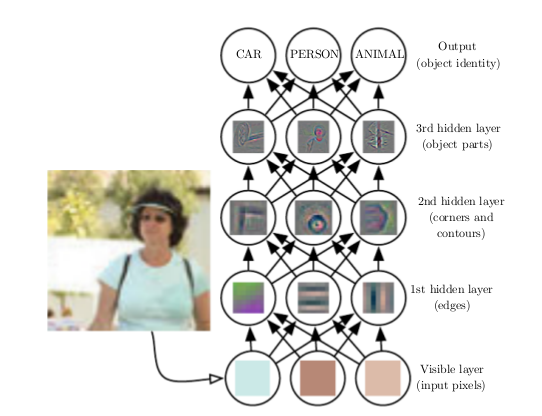
\includegraphics[scale=0.35]{Deep_learning}
	\caption{Ilustrasi cara kerja model \textit{deep learning}}
	\label{Dl_model}
\end{figure}

Gambar \ref{Dl_model} merupakan ilustrasi dari model \textit{deep learning}. Sulit bagi komputer untuk memahami arti dari data input sensoris mentah, seperti gambar tersebut yang direpresentasikan
sebagai kumpulan nilai piksel. Pemetaan fungsi dari sekumpulan piksel itu ke identitas objek sangat rumit. Mempelajari atau mengevaluasi pemetaan ini kemungkinan tidak dapat diatasi jika
ditangani secara langsung. Deep learning menyelesaikan masalah ini dengan memecah pemetaan rumit yang diinginkan ke dalam serangkaian pemetaan sederhana yang bersarang, masing-masing
pemetaan dijelaskan oleh lapisan (layer) model yang berbeda. Input disajikan pada layer yang terlihat \textit{(visible layer)}, dinamakan demikian karena mengandung variabel yang dapat diamati.
Kemudian serangkaian lapisan tersembunyi \textit{(hidden layer)} mengekstraksi fitur yang semakin abstrak dari gambar. Lapisan-lapisan ini disebut "tersembunyi" karena nilainya tidak diberikan
dalam data. Model harus menentukan konsep yang tepat untuk menjelaskan bagaimana hubungan antar data yang sedang diamati. Pada model \textit{deep learning}, data gambar adalah visualisasi dari 
jenis fitur yang diwakili oleh setiap unit hidden layer. Diberikan sebuah data gambar dalam bentuk sekumpulan piksel, lapisan pertama dapat dengan mudah mengidentifikasi tepi dengan cara
membandingkan kecerahan piksel-piksel disekelilingnya. Selanjutnya, output dari \textit{hidden layer} pertama diberikan sebagai input \textit{hidden layer} kedua. \textit{Hidden layer} kedua dapat dengan mudah
mencari sudut dan kontur yang diperpanjang, yang dikenali sebagai koleksi tepi. Mengingat deskripsi \textit{hidden layer} kedua merupakan informasi dalam sudut dan kontur, \textit{hidden layer} ketiga
dapat mendeteksi seluruh bagian dari objek dengan cara menemukan koleksi kontur dan sudut tertentu. Akhirnya, deskripsi fitur dapat digunakan untuk mengenali objek yang ada dalam gambar
\cite{DLConcept}.

\textit{Deep learning} telah mencapai tingkat akurasi yang mendekati manusia dalam berbagai jenis klasifikasi dan tugas prediksi termasuk
gambar, teks, ucapan, dan data video \cite{CODL2018}

\subsection{Long-Short Term Memory (LSTM)}
LSTM merupakan jenis \textit{recurrent neural network} yang dikhususkan untuk memproses suatu data sekuensial misalnya $x^{(1)}, x^{(2)}, ...,x^{(T)}$ \cite{LSTM_2}. 
Berdasarkan gambar \ref{arsi_lstm}, LSTM terdiri atas lapisan input, lapisan output dan lapisan tersembunyi atau \textit{hidden layer}. Lapisan yang berdekatan saling terhubung penuh, sementara tidak ada koneksi di antara node dalam lapisan yang sama.
\textit{Hidden layer} terdiri dari satu set subnet yang terhubung berulang, yang dikenal sebagai blok memori. Tidak seperti lapisan tanh tunggal dalam jaringan RNNs standar, setiap blok memori berisi satu atau lebih sel memori serta tiga gerbang multiplikatif
yaitu \textit{input gate}, \textit{output gate}, \textit{forget gate}. \textit{Input gate} berperan untuk menentukan apakah sinyal yang datang dapat masuk atau tidak serta menghitung seberapa besar sinyal tersebut akan mempengaruhi sel memory.
\textit{Forget gate} menentukan seberapa besar state untuk sel memory sebelumnya dipertahankan atau dilupakan. \textit{Output gate} menentukan seberapa besar state dari memori sel dapat mempengaruhi neuron lainnya \cite{LSTM_1}.

\begin{figure}
	\centering
	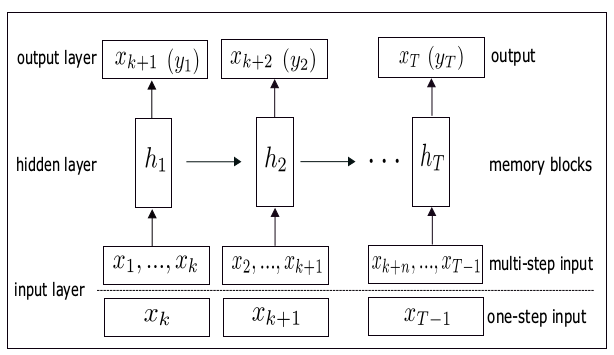
\includegraphics[scale=0.45]{lstm_structure}
	\caption{Struktur LSTM}
	\label{arsi_lstm}
\end{figure}

Dari gambar \ref{arsi_rnn} dapat diketahui bahwa RNN merupakan jaringan feedforward yang sangat dalam dimana semua lapisan memiliki bobot yang sama. Meskipun tujuan utama dari RNN untuk mempelajari dependensi 
jangka panjang, bukti teoritis dan empiris menunjukan bahwa dengan struktur yang demikian, sangat sulit bagi RNN untuk belajar dan meyimpan informasi jangka panjang. Hal ini dikarenakan RNN mengalami masalah yang disebut 
\textit{vanishing gradient} dan \textit{exploding gradient}. Seperti yang kita ketahui dalam proses belajar, sinyal gradien akan terakumulasi sepnjang \textit{hidden layer} dan dikalikan dengan matriks bobot masing-masing neuron.
Jika matriks bobot terlalu kecil maka sinyal gradien akan menjadi terlalu kecil sehingga proses belajar akan terhenti. Sebaliknya, jika matriks bobot terlalu besar menyebabkan sinyal gradien juga terlalu besar sehingga proses belajar menjadi divergen \cite{LSTM_2}

\begin{figure}
	\centering
	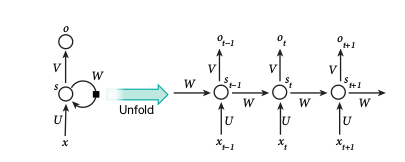
\includegraphics[scale=0.65]{rnn}
	\caption{Struktur RNN}
	\label{arsi_rnn}
\end{figure}

LSTM diciptakan untuk mengatasi masalah \textit{vanishing gradient} dan \textit{exploding gradient} melalui sel memori serta tiga gerbang yang dimilikinya. Secara sigkat, perbedaan mendasar antara RNN dan LSTM dalam proses belajar adalah  RNN menghitung \textit{hidden state} baru dari awal berdasarkan \textit{hidden state} dan input sebelumnya ,sedangkan LSTM menghitung \textit{hidden state} baru dengan memilih apa yang akan ditambahkan ke state saat ini.


\subsubsection{Prediksi menggunakan LSTM}
Sebagai contoh dalam kasus prediksi arus lalu lintas, misalnya runtun nilai input adalah $X = (x_{1},x_{2},...,x_{T})$ , hidden vektor yang terhitung adalah $H = (h_{1},h_{2},...,h_{T})$ dan runtun yang akan diprediksi adalah $Y = (y_{1},y_{2},...,y_{T})$. 
Proses pembaruan setiap timestep $t$ pada lapisan sel memori LSTM dideskripsikan sebagai berikut:
\begin{equation} \label{input_gate}
 i_{t} = \sigma(W_{i}x_{t} + U_{i}c_{t-1}+b_{i})
\end{equation}
\begin{equation} \label{forget_gate}
	f_{t} = \sigma(W_{f}x_{t} + U_{f}c_{t-1}+b_{f})
\end{equation}
\begin{equation} \label{cell_state}
	c_{t} = f_{t}\circ c_{t-1} + i_{t}\circ g(W_{c}x_{t}+b_{c})
\end{equation}
\begin{equation} \label{output_gate}
	o_{t} = \sigma(W_{o}x_{t} + U_{o}c_{t-1}+b_{o})
\end{equation}
\begin{equation} \label{hidden_state}
	h_{t} = o_{t} \circ \sigma_{h}(c_{t})
\end{equation}
\begin{equation} \label{result_gate}
	y_{t} = \phi(W_{y}h_{t} + b_{y})
\end{equation}

Pada persamaan diatas $W_{i}$,$W_{f}$,$W_{c}$, $W_{o}$, $W_{y}$, $U_{i}$,$U_{f}$, $U_{o}$ adalah matiks bobot. Sedangkan $b_{i}$,$b_{f}$, $b_{c}$, $b_{o}$, $b_{y}$ adalah vektor bias.
$\circ$ adalah perkalian \textit{element-wise} dari vektor. $\sigma$, $g$, $\phi$ adalah fungsi aktivasi.

Berdasarkan persamaan \ref{input_gate}, \ref{forget_gate}, \ref{cell_state}, \ref{output_gate}, \ref{hidden_state}, \ref{result_gate}, secara sederhana proses yang terjadi di dalam sel LSTM sebagai berikut. Pertama, $U$ adalah matriks bobot dari masukan $x_{t}$ dan $W$ matriks bobot dari \textit{hidden state} $h_{t}$ yang berulang. 
$f_{t}$ adalah hasil dari komputasi \textit{forget gate}. Dan $i_{t}$ dihitung sebagai \textit{input gate} yang mewakili seberapa banyak penskalaan untuk setiap perubahan pada actual state. 
Selanjutnya, nilai kandidat baru $c_t$ akan dihitung dan merepresentasikan informasi apa yang bisa ditambahkan ke state selanjutnya. 
Sel state selanjutnya akan dihitung sebagai kombinasi informasi apa yang harus dilupakan di hidden state sebelum $c_{t-1}$ dan kandidat skala baru dari $i_{t} \star c_{t}$. 
Terakhir, \textit{hidden state} $h_{t}$ dihitung sama dengan RNN dengan menskalakan menurut cell state baru $c_t$.

\subsubsection{Strategi prediksi menggunakan LSTM}
\paragraph{Strategi \textit{Direct Multi-Step Forecast}}

Metode prediksi secara langsung melibatkan pengembangan model terpisah untuk setiap timestep prediksi seperti yang diilustrasikan persamaan \ref{direct_forcast} \cite{Forecast_Strategy}.
Sebagai contoh, memprediksi suhu untuk dua hari ke depan. Maka dikembangkan model untuk memprediksi suhu pada hari ke-1 dan model terpisah untuk memprediksi suhu pada hari ke-2.
\begin{equation} \label{direct_forcast}
\begin{bmatrix}
	prediction(t+1) = model1[data(t-1), data(t-2), ..., data(t-n)]
	\\prediction(t+2) = model2[data(t-2), data(t-3), ..., data(t-n)]
\end{bmatrix}
\end{equation}

Karena terdapat satu model untuk tiap timestep, hal ini akan menambah beban komputasi dan beban maintenance model terutama ketika jumlah timestep yang akan diprediksi meningkat. Selain itu
karena terdapat model yang terpisah berarti hubungan dependensi antar hasil prediksi tidak dapat dimodelkan.

\paragraph{Strategi \textit{Recursive Multi-Step Forecast}} 

Strategi rekursif melibatkan penggunaan model satu timestep secara berulang beberapa kali. Seperti pada persamaan \ref{recursive_forcast} hasil prediksi timestep sebelumnya akan digunakan sebagai input untuk melakukan prediksi pada timestep selanjutnya \cite{Forecast_Strategy}.
Dalam hal memprediksi suhu untuk dua hari ke depan, maka dikembangkan model prediksi cukup satu timestep. Model ini kemudian akan digunakan untuk memprediksi hari 1, hasil prediksi hari 1 ini akan digunakan sebagai input pengamatan untuk memprediksi hari 2.
\begin{equation} \label{recursive_forcast}
\begin{bmatrix}
		prediction(t+1) = model[data(t-1), data(t-2), ..., data(t-n)]
		\\prediction(t+2) = model[prediction(t+1), data(t-1), ..., data(t-n)]
\end{bmatrix}
\end{equation}

Karena menggunakan prinsip hasil prediksi digunakan sebagai input pengamatan selanjutnya, strategi rekursif memungkinkan kesalahan prediksi terakumulasi sedemikian rupa sehingga kinerja model dapat dengan cepat menurun ketika timestep yang akan diprediksi meningkat.

\paragraph{Strategi \textit{Direct-Recursive Hybrid}}

Strategi langsung dan rekursif dapat digabungkan untuk menawarkan manfaat dari kedua metode.
Seperti pada persamaan \ref{hybrid_forcast}, model terpisah dapat dibuat untuk tiap timestep yang akan diprediksi, tetapi masing-masing model dapat menggunakan hasil prediksi yang dibuat oleh model lain pada timestep sebelumnya sebagai nilai input \cite{Forecast_Strategy}.
\begin{equation} \label{hybrid_forcast}
\begin{bmatrix}
		prediction(t+1) = model1[data(t-1), data(t-2), ..., data(t-n)]
		\\prediction(t+2) = model2[prediction(t+1), data(t-1), ..., data(t-n)]
\end{bmatrix}
\end{equation}

Menggabungkan strategi rekursif dan langsung dapat membantu mengatasi keterbatasan masing-masing metode.

\paragraph{Strategi \textit{Multi Output}}

Strategi multi-output melibatkan pengembangan satu model yang mampu memprediksi seluruh runtun prediksi yang diinginkan dalam satu langkah \cite{Forecast_Strategy}.
Dalam hal memprediksi suhu untuk dua hari ke depan, seperti pada persamaan \ref{MIMO_forcast} satu model digunakan untuk memprediksi suhu dua hari berikutnya dalam satu operasi.
\begin{equation} \label{MIMO_forcast}
		prediction(t+1), prediction(t+2) = model[data(t-1), ..., data(t-n)]
\end{equation}

Model multi output lebih kompleks karena model ini dapat mempelajari struktur ketergantungan antara input dan output serta antara output satu dengan output yang lain.
Oleh karena itu model ini membutuhkan waktu lebih banyak untuk proses belajar serta membutuhkan lebih banyak data untuk menghindari \textit{overfitting}.

\subsubsection{Indikator Kesalahan Hasil Prediksi menggunakan LSTM}
Kesalahan \textit{(Error)} merupakan nilai selisih antara nilai sesungguhnya dengan nilai hasil prediksi. Semakin besar nilai kesalahan maka dapat dikatakan bahwa akurasi model prediksi 
yang digunakan rendah. Terdapat tiga indikator kesalahan yang umum dipakai untuk mengevaluasi hasil prediksi LSTM \cite{LSTM_2}:

\paragraph{\textit{Mean Squared Error}  (MSE)} 

\textit{Mean Squared Error} merupakan rata-rata nilai kuadrat selisih antara nilai sebenarnya $y_i$ dengan nilai hasil prediksi $y^{'}_i$ sejumlah T waktu. Secara matematis dapat dituliskan pada persamaan \ref{MSE}
\begin{equation}\label{MSE}
	MSE = \frac {1}{T}\sum \limits_{i=1}^{T} {(y_i - y^{'}_i)^2}
\end{equation}

Dengan adanya operasi kuadrat pada selisih nilai sebenarnya dengan nilai prediksi, maka nilai kesalahan akan selalu positif. Namun, operasi kuadrat ini juga membuat nilai kesalahan 
akan semakin besar jika selisih nilai sebenarnya dengan nilai prediksi juga besar.


\paragraph{\textit{Root Mean Squared Error} (RMSE)}

\textit{Root Mean Squared Error} adalah akar kuadrat dari rata-rata nilai kuadrat selisih antara nilai sebenarnya $y_i$ dengan nilai hasil prediksi $y^{'}_i$ sejumlah T waktu seperti pada persamaan \ref{RMSE}
\begin{equation}\label{RMSE}
	RMSE = \sqrt{\frac {1}{T}\sum \limits_{i=1}^{T} {(y_i - y^{'}_i)^2}}
\end{equation}

Operasi akar pada RMSE mengakibatkan hasil dari nilai kesalahan akan memiliki skala nilai yang sama dengan nilai realisasi ataupun nilai peramalan, sehingga
indikator RMSE lebih mudah dipahami daripada indikator MSE. 

\paragraph{\textit{Mean Absolute Percentage Error} (MAPE)}

Mean Average Percentage Error (MAPE) adalah persentase rata-rata perbandingan selisih antara nilai sebenarnya $y_i$ terhadap nilai hasil prediksi $y^{'}_i$ sejumlah T
titik waktu seperti pada persamaan \ref{MAPE}
\begin{equation}\label{MAPE}
	MAPE = \sqrt{\frac {100}{T}\sum \limits_{i=1}^{T} {\left|{\frac {y_i - y^{'}_i}{y_i}}\right|}}
\end{equation}

Tampilan persen pada MAPE memberikan kemudahan dalam perhitungan akurasi. Akan tetapi, MAPE tidak disarankan untuk digunakan jika nilai sebenarnya $y_i$
bernilai nol, hal ini dikarenakan saat nilai sebenarnya $y_i$ nol maka penyebut pada persamaan akan bernilai nol, sehingga nilai kesalahan akan menjadi tidak berhingga.

\subsection{\textit{Convolutional Neural Network} (CNN)}

\textit{Convolutional Neural Network} (CNN) adalah salah satu jenis neural network yang biasa digunakan pada data gambar. CNN bisa digunakan untuk mendeteksi dan mengenali objek pada sebuah gambar.
CNN tidak jauh berbeda dengan \textit{neural network} pada umumnya. CNN terdiri dari neuron yang memiliki bobot, bias dan fungsi aktivasi \cite{Wu2017IntroductionTC}.

Seperti pada gambar \ref{arsi_CNN}, arsitektur CNN dibagi menjadi dua yaitu \textit{Feature Extraction Layer} dan \textit{Fully-Connected Layer} (FCN). \textit{Feature Extraction Layer} terdiri dari lapisan konvolusi dan lapisan \textit{pooling}.
\begin{figure}[htp]
	\centering
	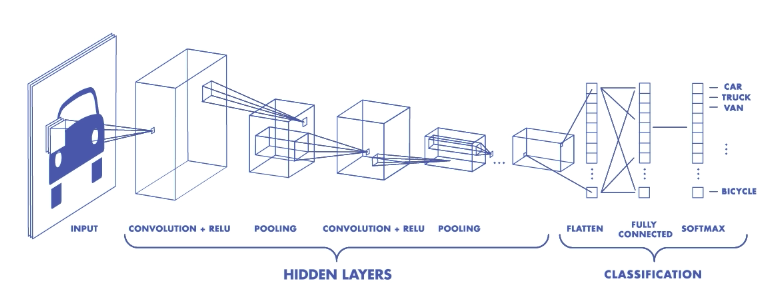
\includegraphics[scale=0.5]{CNN}
	\caption{Arsitektur CNN}
	\label{arsi_CNN}
\end{figure}

\subsubsection{Lapisan Konvolusi}
Lapisan konvolusi merupakan lapisan dimana fitur dari input akan diekstrak menggunakan sebuah filter yang mempunyai ukuran tertentu. Lapisan konvolusi hanya dapat
dioperasikan pada input yang memliliki minimal dua dimensi. Parameter dari lapisan konvolusi yang paling umum adalah filter, ukuran filter, stride, dan padding \cite{Wu2017IntroductionTC}.

\paragraph{Filter}

Filter berupa matriks dan digunakan dalam proses konvolusi \cite{Wu2017IntroductionTC}. Proses konvolusi dilakukan dengan menggeser filter sepanjang data input seperti yang diilustrasikan pada gambar \ref{konvolusi_CNN}. Besarnya pergeseran ditentukan oleh nilai stride yang digunakan. Pada setiap pergeseran, dilakukan operasi perkalian matriks antara elemen input dengan elemen filter. Hasil perkalian tersebut kemudian dijumlahkan dan 
disimpan pada fitur map. Matriks filter konvolusi umumnya menggunakan ukuran 3 x 3 atau 5 x 5. Ukuran dari matriks filter harus ganjil untuk memudahkan proses konvolusi hal iini dikarenakan proses konvolusi membutuhkan satu elemen center, sedangkan pada matriks dengan ukuran genap, tidak ada elemen yang merupakan center dari matriks.

\begin{figure}[htp]
	\centering
	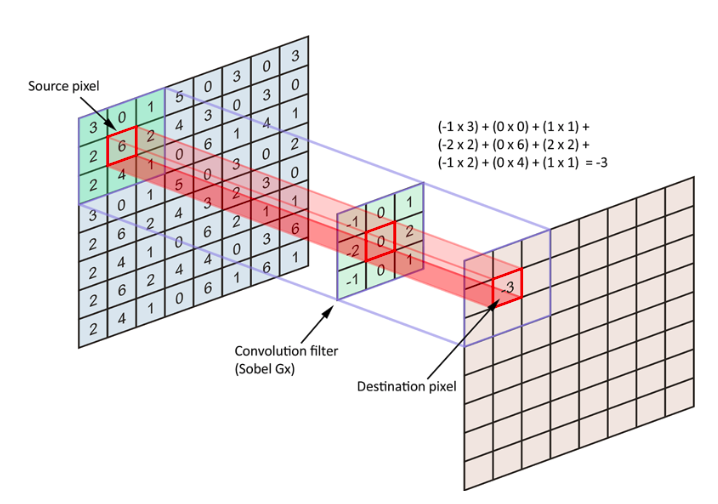
\includegraphics[scale=0.3]{filter_cnn}
	\caption{Ilustrasi proses konvolusi pada CNN}
	\label{konvolusi_CNN}
\end{figure}

\paragraph{Stride}

Stride adalah parameter yang menentukan berapa jumlah pergeseran filter. Jika nilai stride adalah 1, maka filter konvolusi akan bergeser sebanyak 1 pixels secara horizontal lalu vertical \cite{KarpathyCNN}. 
Semakin kecil stride maka akan semakin detail informasi yang kita dapatkan dari sebuah input, namun membutuhkan komputasi yang lebih jika dibandingkan dengan stride yang besar.

\paragraph{Padding}

Sedangkan Padding atau Zero Padding adalah parameter yang menentukan jumlah pixels (berisi nilai 0) yang akan ditambahkan di setiap sisi dari input seperti pada gambar \ref{padding_CNN}. Hal ini digunakan dengan tujuan untuk memanipulasi dimensi output dari lapisan konvolusi (fitur map) \cite{KarpathyCNN}.
Dimensi output dari lapisan konvolusi selalu lebih kecil dari inputnya (kecuali penggunaan 1x1 filter dengan stride 1). Output ini akan digunakan kembali sebagai input dari lapisan konvolusi selanjutnya, sehingga tentu saja semakin banyak informasi yang terbuang.
Dengan menggunakan padding, dimensi output dapat diatur agar tetap sama seperti dimensi input atau setidaknya tidak berkurang secara drastis. Dengan demikian kita bisa menggunakan lapisan konvolusi yang lebih dalam/\textit{deep} sehingga lebih banyak fitur yang berhasil diekstrak.

\begin{figure}[htp]
	\centering
	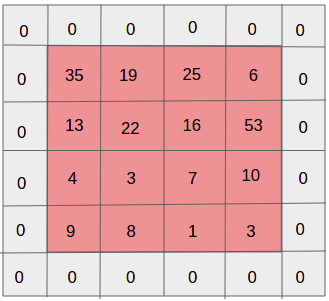
\includegraphics[scale=0.45]{padding}
	\caption{Ilustrasi penerapan padding pada CNN}
	\label{padding_CNN}
\end{figure}

Persamaan \ref{Fitur_map_dim} menghitung dimensi dari fitur map berdasarkan ukuran filter, stride dan padding yang digunakan.
\begin{equation}\label{Fitur_map_dim}
	output =\frac {W-N-2P}{S}+1
\end{equation}
dimana $W$ : dimensi input, $N$ : ukuran filter, $P$ : padding, dan $S$ : stride


\subsubsection{Lapisan \textit{Pooling}}
Fungsi dari lapisan \textit{pooling} ini adalah untuk mengurangi dimensi dari fitur map secara spasial (mengurangi jumlah
parameter) dengan operasi \textit{down-sampling} \cite{CNNinImageNet}. Proses \textit{pooling} ditunjukan oleh gambar \ref{pooling_CNN}. Dengan pooling 2 x 2 stride 2, jumlah parameter akan direduksi sebanyak 75\%, sangat berguna untuk mengurangi kebutuhan komputasi. Selain
mereduksi jumlah parameter, pooling juga berfungsi untuk mencegah \textit{overfitting}.

Umumnya, metode \textit{pooling} yang digunakan adalah \textit{max pooling} atau mengambil nilai terbesar dari suatu bagian/daerah. Namun terdapat metode pooling lain yang dapat digunakan seperti \textit{average pooling} atau
\textit{L2-norm pooling} \cite{CNNinImageNet}.
\begin{figure}[htp]
	\centering
	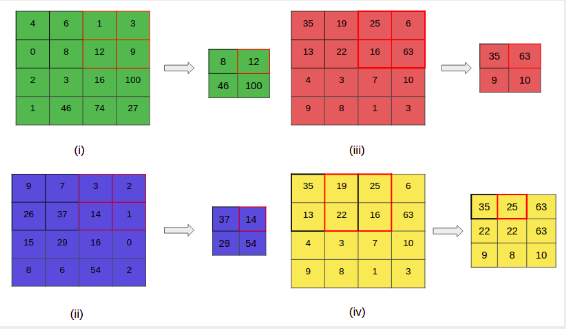
\includegraphics[scale=0.45]{pooling}
	\caption{Ilustrasi proses \textit{pooling} pada CNN}
	\label{pooling_CNN}
\end{figure}

\subsubsection{\textit{Fully-Connected Layer} (FCN)}
Fitur map yang dihasilkan dari \textit{feature extraction layer} masih berbentuk multidimensional array, sehingga harus dilakukan “flatten” atau reshape terhadap fitur map menjadi sebuah vector agar bisa digunakan sebagai input dari \textit{fully-connected layer}.

\textit{Fully-connected layer} berfungsi sebagai \textit{classifier} berdasarkan fitur map yang telah diekstrak dari input. FCN akan memberikan probabilitas untuk tiap objek pada gambar.

\subsection{YOLO (\textit{You Only Look Once}) V3}

\textit{You Only Look Once} (YOLO) merupakan suatu metode pendekatan yang bertujuan untuk deteksi objek. YOLO melihat deteksi objek sebagai suatu masalah regresi dari \textit{bounding box} dan
probabilitas kelas yang terpisah secara spasial. YOLO merupakan \textit{neural network} yang memprediksi \textit{bounding box} dan \textit{class probability} dari gambar utuh secara langsung dalam satu kali
evaluasi. Oleh karena deteksi YOLO menggunakan \textit{single network}, maka optimasi performa deteksi dapat dilakukan langsung secara end-to-end \cite{YoloV1}.

Secara arsitekturnya, YOLO hanya menggunakan lapisan konvolusi sehingga menjadikannya sebuah jaringan konvolusi penuh (FCN). Pada YOLOV3 terdapat 75 lapisan konvolusi dengan \textit{skip connection} dan lapisan upsampling.
YOLOv3 menggunakan stride 2 untuk \textit{downsample} fitur map serta tidak menggunakan lapisan \textit{pooling} untuk mencegah hilangnya informasi dari fitur tingkat rendah. Pada YOLOV3 setiap \textit{bounding box} memiliki atribut array ukuran \textbf{(5 + C)} dimana array ini mengandung informasi
mengenai koordinat titik tengah, ukuran dimensi, skor objektivitas, dan $C$ skor kelas.

YOLOV3 mendeteksi suatu objek dengan cara membagi gambar input kedalam grid sebanyak ukuran fitur map. Kemudian masing-masing grid akan memprediksi \textit{bounding box} sebanyak 3 buah.
Kemudian jaringan akan mencari grid yang berpotensi memiiliki koordinat titik tengah suatu objek pada gambar input. Grid-grid tersebutlah yang kemudian akan bertanggung jawab untuk melakukan prediksi \textit{bounding box} untuk objek \cite{YoloV3}.

Sebagai contoh, misalkan suatu gambar input berukuran 416x416 dan stride pada lapisan deteksi bernilai 32, maka fitur map akan memiliki dimensi 13x13. Selanjutnya gambar input akan dibagi menjadi 13 grid seperti pada gambar \ref{grid_YOLO}.
\begin{figure}
	\centering
	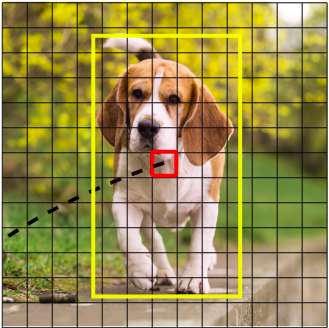
\includegraphics[scale=0.5]{grid_input}
	\caption{Gambar input dibagi kedalam grid sesuai ukuran fitur map}
	\label{grid_YOLO}
\end{figure}
Berdasarkan gambar \ref{grid_YOLO}, grid yang berpotensi memiliki koordinat titik tengah objek adalah grid merah (baris dan kolom ke-7). Berarti, grid inilah yang bertugas untuk memprediksi \textit{bounding box} dari objek (anjing). 

YOLO memprediksi titik tengah \textit{bounding box} dengan mencari offset relatif terhadap grid pojok kiri atas dari grid yang bertugas untuk memprediksi \cite{YoloV2}. Pada contoh diatas, grid yang digunakan sebagai acuan adalah grid (6,6).
Persamaan untuk mencari \textit{bounding box}:
\begin{equation} \label{bx_bb}
	b_{x} = \sigma(t_{x}) + c_x
   \end{equation}
\begin{equation} \label{by_bb}
	b_{y} = \sigma(t_{y}) + c_y
\end{equation}
\begin{equation} \label{bw_bb}
	b_{w} = p_{w}e^{t_w}
\end{equation}
\begin{equation} \label{bh_bb}
	b_{h} = p_{h}e^{t_h}
\end{equation}
$b_x$, $b_y$: koordinat titik tengah pada gambar input, $b_w$, $b_h$: lebar dan tinggi hasil prediksi, $t_x$, $t_y$: koordinat titik tengah terhadap grid, $t_w$, $t_h$: lebar dan tinggi terhadap grid, $c_x$, $c_y$: grid acuan (pojok kiri atas), pada contoh diatas grid (6,6). Sedangkan $p_h$, $p_w$: dimensi anchor box yang digunakan. 
$t_x$, $t_y$ dilewatkan fungsi sigmoid agar nilainya berada diantara 0 dan 1. Hal ini agar koordinat titik tengah hasil prediksi tidak keluar dari grid yang bertugas melakukan prediksi, dalam contoh diatas yaitu grid (7,7)

Skor kelas menunjukan probabilitas objek yang terdeteksi milik kelas tertentu. Pada YOLO, dan YOLOV2 skor kelas menggunakan softmax, sedangkan pada YOLOV3 menggunkan sigmoid.
Skor kelas yang dihitung menggunakan softmax mengasumsikan bahwa kelas-kelas tersebut saling eksklusif. Dengan kata lain, jika suatu objek telah terdeteksi milik satu kelas, maka dijamin tidak bisa milik kelas lain. 
Namun, asumsi ini kurang cocok digunakan ketika memiliki 2 atau lebih kelas dengan fitur yang hampir mirip, sebagai contoh kelas wanita dan orang. Oleh karena inilah, YOLOV3 mengunakan sigmoid untuk skor kelas \cite{YoloV3}.

Terdapat beberapa hal yang membuat YOLOV3 lebih baik dibandingkan objek detector lainnya yaitu: Anchor Box, \textit{Intersection over Union}(IoU), \textit{Non-Maxima Supression}(NMS) dan Fitur Ekstraktor.
\subsubsection{Anchor Box}
Anchor box adalah beberapa bentuk \textit{bounding box} yang telah didefinisakan sebelumnya yang mewakili bentuk objek pada dataset. Anchor box memudahkan dan mempercepat proses prediksi \textit{bounding box} terutama pada kasus dimana terdapat dua objek atau lebih berada di satu grid yang sama sehingga titik tengah kedua objek juga terletak pada grid yang sama seperti pada gambar \ref{anchor_box_merge}. 
Tanpa menggunakan anchor box, sangat sulit untuk mendapatkan 2 \textit{bounding box} dalam satu grid.

\begin{figure}[htp]
	\centering
	\begin{subfigure}{0.4\textwidth}
	  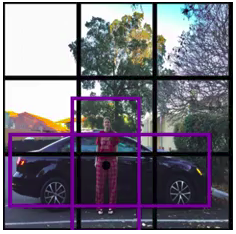
\includegraphics[width=\textwidth]{anchor.png}
	  \caption{}
	  \label{ancor}
	\end{subfigure}
	\begin{subfigure}{0.4\textwidth}
	  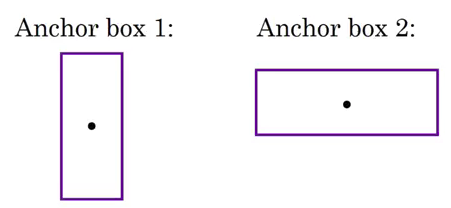
\includegraphics[width=\textwidth]{anchor_box.png}
	  \caption{}
	  \label{anchor_box}
	\end{subfigure}
	\caption{Anchor box untuk memudahkan prediksi \textit{bounding box}}
	\label{anchor_box_merge}
  \end{figure}

Objek dikelompokan ke anchor box berdasarkan kesamaan bentuk \textit{bounding box} objek tersebut dengan anchor box. Untuk gambar \ref{anchor_box_merge}, kelas orang akan masuk anchor box 1, sedangkan kelas mobil masuk anchor box 2.

Pada YOLOV3, lapisan deteksi memiliki stride berukuran 32,16,8. Artinya, untuk input gambar 416x416 maka akan dilakukan deteksi pada 3 skala berbeda yaitu 13x13, 26x26, dan 52x52. Hal ini biasa disebut prediksi lintas skala.
Pada YOLOV3, tiap grid di tiap skala memprediksi 3 \textit{bounding box} menggunakan 3 anchor. Sehingga untuk 3 skala, YOLOV3 membutuhkan 9 anchor box. Pada dataset COCO, 9 anchor box itu antara lain: (10 × 13), (16 × 30), (33 × 23), (30 × 61), (62 × 45), (59 ×
119), (116 × 90), (156 × 198), (373 × 326) \cite{YoloV3}.

Diatas juga telah disebutkan bahwa pada YOLOV3 setiap \textit{bounding box} memiliki atribut array ukuran \textbf{(5 + C)}. Apabila dijumlahkan secara total, label untuk gambar 416x416 memiliki ukuran $((52x52)+(26x26)+(13x13))\star 3 \star (5+C)$

\subsubsection{\textit{Intersection over Union}(IoU)}
Seperti yang telah dijelaskan, YOLOV3 memprediksi 3 \textit{bounding box} pada tiap grid. Untuk dapat menentukan manakah \textit{bounding box} yang paling bagus dari ketiga \textit{bounding box} yang ada, maka digunakan \textit{Intersection over Union}(IoU). 
IoU akan membandingkan kesamaan antara dua bentuk dengan cara menghitung seberapa besar kedua bentuk tersebut bersimpangan \cite{IoU}.
\begin{equation} \label{IoU}
	IoU = \frac{|A \cap B|}{|A \cup B|}	\hspace{10mm} untuk \hspace{1mm}A,B \subseteq \mathbb{S} \in \mathbb{R}^n
\end{equation}

Berdasarkan persamaan \ref{IoU}, IoU dihitung berdasakan luasan daerah yang bersimpangan terhadap total luasan daerah.
Dalam konteks objek deteksi, maka IoU dihitung dengan membandingkan antara \textit{bounding box} hasil prediksi dengan \textit{bounding box groundtruth}.

\subsubsection{\textit{Non-Maxima Supression}(NMS)}
Pada konteks objek deteksi, Non-Maxima Supression (NMS) digunakan untuk menyaring \textit{bounding box} untuk diambil yang memiliki IoU terbesar dan meniadakan \textit{bounding box} yang lain. 
Teknik ini sangat bermanfaat apabila terdapat lebih dari satu \textit{bounding box} dalam satu objek. NMS akan memastikan bahwa untuk tiap objek hanya ada satu buah \textit{bounding box}. 

Secara singkat, cara kerja NMS sebagai berikut:
\begin{enumerate}
	\item Eliminasi semua \textit{bounding box} yang memiliki IoU kurang dari atau sama dengan yang telah ditetapkan.
	\item Untuk \textit{bounding box} yang tersisa
	\begin{enumerate}
		\item Ambil \textit{bounding box} yang memiliki IoU terbesar. \textit{Bounding box} inilah yang menjadi output prediksi.
		\item Hilangkan \textit{bounding box} yang lain.
	\end{enumerate}
	\item Ulangi langkah 2 sampai semua \textit{bounding box} untuk tiap objek telah diperoleh.
\end{enumerate}

\subsubsection{Fitur Ekstraktor}
YOLOV3 menggunakan Darknet-53 sebagai fitur ekstraktor. Darknet-53 memiliki 53 lapisan konvolusi seperti pada gambar \ref{darknet_53}.
\begin{figure}[htp]
	\centering
	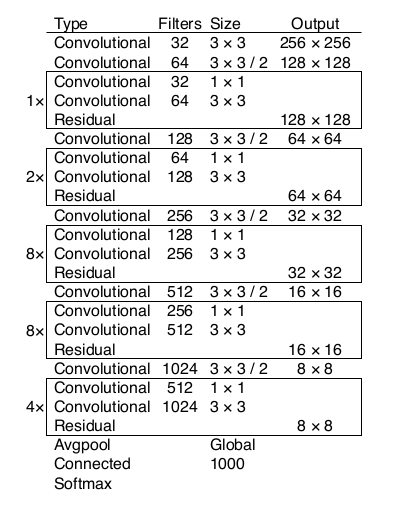
\includegraphics[scale=0.5]{darknet_53}
	\caption{Arsitektur Darknet-53}
	\label{darknet_53}
\end{figure}
Darknet-53 lebih powerful dibandingkan Darknet-19 \cite{YoloV2}, dan lebih efisien daripada ResNet-101 atau ResNet-152 \cite{YoloV3}.

Pengukuran pada tabel \ref{tabel_comp_FE} \cite{YoloV3} pada GPU Titan X dengan ukuran input 256 × 256. Berdasarkan tabel tersebut dapat dilihat bahwa Darknet-53 memiliki performa setara dengan fitur ekstraktor lain tetapi dengan operasi \textit{floating point} lebih sedikit dan kecepatan lebih tinggi. Darknet lebih cepat 1.5 kali daripada ResNet-101 dan 2 kali daripada ResNet-152.
Darknet-53 juga memiliki nilai operasi \textit{floating point} per detik paling tinggi. Hal ini menunjukan bahwa arsitektur yang dimiliki yang mana didominasi oleh lapisan konvolusi sangat efisien berjalan di GPU, sehingga membuat eksekusi Darknet-19 lebih cepat \cite{YoloV3}.

\begin{table}[htp]
\centering
\begin{tabular}{ cccccc } 
	Backbone & Top-1 & Top5 & Bn Ops & BFLOP/s & FPS\\
	\hline
	Darknet-19 \cite{YoloV2} & 74.1& 91.8& 7.29& 1246 & 171\\
	ResNet-101 \cite{ResNet} & 77.1& 93.7& 19.7& 1039 & 53 \\
	ResNet-152 \cite{ResNet} & 77.6& 93.8 &29.4& 1090 & 37 \\
	Darknet-53 \cite{YoloV3} &77.2& 93.8&18.7& 1457 & 78 \\
\end{tabular}
\caption{Perbandingan performa berbagai fitur ekstraktor}
\label{tabel_comp_FE}
\end{table}

\subsection{Kalman Filter}

Kalman filter adalah persamaan matematika sebagai alat komputasi efisien (rekursif) untuk memperkirakan atau mengestimasi \textit{state} dari suatu proses dengan meminimalkan \textit{mean squared error}.
Komponen dasar Kalman Filter adalah vektor \textit{state}, model dinamis dan model observasi.
Vektor \textit{state} menggambarkan \textit{state} dari sistem dinamis dan menunjukkan derajat kebebasan. Varabel di vektor \textit{state} dapat berupa posisi, kecepatan, orientasi sudut dasn sebagainya. Vektor \textit{state} memiliki dua nilai pada saat yang sama yaitu 
nilai yang diprediksi sebelum di\textit{update} dan nilai posterior setelah di\textit{update} \cite{Kalman}.

Model Kalman Filter mengasumsikan \textit{state} yang benar pada waktu $k$ didapatkan dari \textit{state} pada waktu $k-1$ menurut persamaan \ref{Kalman_Filter}.
\begin{equation} \label{Kalman_Filter}
	\textbf{x}_k = \textbf{F}_{k}\textbf{x}_{k-1} + \textbf{B}_{k}\textbf{u}_k + \textbf{w}_k
\end{equation}
dimana $\textbf{F}_{k}$: model transisi \textit{state} yang berlaku pada \textit{state} terdahulu $\textbf{x}_{k-1}$. $\textbf{B}_{k}$: model \textit{control-input} yang berlaku pada vektor kontrol $\textbf{u}_k$.
$\textbf{w}_k$ adalah derau yang terjadi dalam proses yang diasumsikan berdistribusi normal dengan \textit{mean} nol dan \textit{covariance} $\textbf{Q}_k$. 
Pada waktu $k$ sebuah pengamatan atau pengukuran $\textbf{z}_k$ pada \textit{state} sebenarnya dari $\textbf{x}_k$ dibuat berdasarkan persamaan \ref{Kalman_Filter_2}

\begin{equation} \label{Kalman_Filter_2}
	\textbf{z}_k = \textbf{H}_{k}\textbf{x}_{k} + \textbf{v}_k
\end{equation}
dimana $\textbf{H}_k$ adalah model pengamatan yang memetakan \textit{state} yang sebenarnya dan $\textbf{v}_k$ adalah \textit{noise} pengamatan yang diasumsikan sebagai \textit{white gaussian noise} dengan \textit{mean} nol dan \textit{covarian} $\textbf{R}_k$.$\textbf{v}_k \sim N(0, \textbf{R}_k)$. 

Kalman Filter memiliki dua fase yaitu \textbf{\textit{predict}} dan \textbf{\textit{update}}. Fase \textit{predict} memanfaatkan perkiraan waktu sebelumnya untuk memproduksi perkiraan \textit{state} sekarang.
Pada fase \textit{update} informasi yang telah diukur dari waktu sekarang digunakan untuk memperbaiki prediksi guna menghasilkan perkiraan yang akurat \cite{TrackingKalman}. Persamaan untuk \textit{update} dan \textit{update} ditunjukkan oleh \ref{Kalman_predict} dan \ref{Kalman_update}.
\begin{equation} \label{Kalman_predict}
	X(n) = F \cdot X(n-1) + V_{q}(n-1)	
\end{equation}

\begin{equation} \label{Kalman_update}
	Y(n) = H \cdot X(n) + V_{p}(n)
\end{equation}
dimana $X(n)$ dan $Y(n)$ adalah variabel estimasi \textit{state} dan variabel pengukuran. $F$ adalah matriks transisi \textit{state} dan $H$ adalah matriks pengukuran. Sedangkan $V_{q}(n)$ dan $V_{p}(n)$ adalah derau sistem dan derau pengukuran.


\subsection{\textit{K-Nearest Neighbors}}
\textit{K-Nearest Neighbors} (K-NN) adalah metode non parametrik yang digunakan baik untuk klasifikasi maupun regresi. Untuk klasifikasi, output K-NN berupa keanggotaan kelas. Objek diklasifikasikan berdasarkan voting pluralitas dari tetangganya. Objek akan dilabeli sebagai anggota kelas yang paling umum dari $k$ tetangga terdekatnya.
K-NN untuk klasifikasi memiliki 2 tahapan yaitu pertama menentukan tetangga terdekat sebanyak $k$, dan kedua menentukan kelas objek berdasarkan tetangganya \cite{KNN}. 
K-NN melakukan klasifikasi dengan proyeksi data pembelajaran pada ruang berdimensi banyak. Ruang ini dibagi menjadi bagian-bagian yang merepresentasikan kriteria data pembelajaran. Setiap data pembelajaran direpresentasikan menjadi titik-titik $c$ pada ruang dimensi banyak.
Apabila terdapat data baru yang akan diklasifikasi, maka K-NN akan mencari sejumlah tetangga yang memiliki kemiripan dengan data baru kemudian data baru akan diklasifikasi sesuai label tetangga tersebut. 
Proses mencari kemiripan ini menggunakan metric jarak. Metric yang umum dipakai adalah \textit{Euclidean distance} (formula untuk mencari jarak antara 2 titik dalam ruang dua dimensi) dan \textit{Minkowski Distance} \cite{KNN}. Untuk variabel diskrit seperti klasifiksi teks, digunakan metric lain seperti \textit{Hamming distance}.
Persamaan untuk \textit{Euclidean distance} seperti persamaan \ref{Euclidean_Dist}
\begin{equation} \label{Euclidean_Dist}
	d = \sqrt{(x_2 - x_1)^2 + (y_2 - y_1)^2}
\end{equation}
dimana $x_1$ dan $y_1$ adalah koordinat $c$ lama, sedangkan $x_2$ dan $y_2$ adalah koordinat $c$ baru. 

Untuk menggunakan algoritma K-NN, perlu ditentukan banyaknya $k$ tetangga terdekat yang digunakan untuk melakukan klasifikasi data baru.
Penentuan nilai $k$ dipertimbangkan berdasarkan banyaknya data yang ada dan ukuran dimensi yang dibentuk oleh data. Semakin banyak data yang ada, nilai $k$ yang dipilih sebaiknya semakin rendah. Namun, semakin besar ukuran dimensi data, nilai $k$ yang dipilih sebaiknya semakin tinggi.


\subsection{Software penunjang}
\subsubsection{PyTorch}
PyTorch adalah package komputasi berbasis Python yang memanfaatkan GPU. PyTorch merupakan salah satu platform populer untuk penelitian \textit{deep learning} karena memberikan fleksibilitas dan kecepatan yang maksimum.
PyTorch memiliki dua fitur utama yaitu: komputasi Tensor dengan GPU dan memberikan fasilitas untuk membangun \textit{deep neural network} berdasarkan sistem autograd \cite{PyTorch}. 
\begin{figure}[htp]
	\centering
	
\includegraphics[scale=0.2]{PyTorch}
	\caption{PyTorch}
	\label{PyTorch}
\end{figure}


Fitur lain dari PyTorch antara lain:
\begin{enumerate}
	\item \textbf{Interface yang simpel} : PyTorch menawarkan API yang mudah dioperasikan seperti Python
	\item \textbf{\textit{Pythonic in nature}} : Library ini terintegrasikan dengan package \textit{data science} Python. Dengan demikian PyTorch dapat memanfaatkan semua layanan dan fungsi yang ditawarkan oleh Python.
	\item \textbf{Graph komputasi} : PyTorch menawarkan komputasi graph yang dinamis sehingga graph dapat diubah-ubah saat runtime. Hal ini sangat berguna ketika kita tidak mengetahui seberapa banyak memori yang diperlukan untuk membuat model \textit{neural network}.
\end{enumerate}


\subsubsection{Keras}
Keras merupakan high-level neural network API (Application Programming Interface), yang ditulis dengan bahasa pemrograman Python dan mampu berjalan di atas TensorFlow, CNTK, atau
Theano. Keras pertama kali dikembangkan sebagai bagian dari proyek penelitian ONEIROS(Open-ended Neuro-Electronic Intelligent Robot Operating System). Keras dikembangkan dengan
berfokus pada eksperimen cepat. Menuangkan ide dengan cepat merupakan langkah yang baik dalam penelitian. Keras dapat digunakan apabila sistem membutuhkan library deep learning yang
memiliki kriteria sebagai berikut:
\begin{itemize}
	\item Memungkinkan pembuatan prototipe yang mudah dan cepat (melalui fitur kemudahan pengguna, modularitas, dan ekstensibilitas).
	\item Mendukung convolutional network dan recurrent network, serta kombinasi keduanya.
	\item Berjalan mulus di CPU dan GPU.
  \end{itemize}

Keras kompatibel dengan Python 2.7-3.6. Pada penerapannya, keras mempunyai beberapa
kelebihan sebagai berikut:
\begin{enumerate}
	\item \textbf{User friendly}. Keras adalah API yang dirancang untuk manusia, bukan mesin. Keras menawarkan API yang konsisten dan sederhana, serta meminimalkan jumlah action
	pengguna yang diperlukan untuk kasus yang umum. Selain itu, keras memberikan umpan balik yang jelas dan dapat ditindaklanjuti atas kesalahan pengguna.
	\item \textbf{Modularity}. Model dipahami sebagai urutan atau grafik dari modul mandiri \textit{(standalone)}
	yang dapat dikonfigurasi sepenuhnya dan dapat berjalan dengan batasan \textit{(restriction)} yang sederhana. Secara khusus, lapisan saraf \textit{(neural layer)}, fungsi biaya \textit{(cost functions)}, pengoptimalisasi \textit{(optimizers)}, skema inisialisasi \textit{(initialization schemes)}, fungsi aktivasi
	\textit{(activation functions)}, dan skema regularisasi (regularization schemes) adalah modul-modul mandiri yang dapat digabungkan untuk membuat model baru.
	\item \textbf{Easy extensibility}. Modul baru mudah ditambahkan sehingga membuat Keras cocok untuk penelitian lanjutan.
	\item \textbf{Menggunakan bahasa pemrograman Python}. Tidak ada file konfigurasi model
	terpisah dalam format deklaratif. Model dijelaskan dalam kode Python yang kompak,
	lebih mudah untuk di-debug, dan memungkinkan kemudahan ekstensibilitas.
\end{enumerate}

\subsubsection{Dash dari Plotly}
Dash adalah framework berbasis Python untuk membuat aplikasi web. Dash ditulis menggunakan Flask, Plotly.js, dan React.js sehingga sangat cocok untuk membuat aplikasi visualisasi data dengan \textit{user interface} sesuai keinginan dan murni menggunakan Python. 
Dash dirender di web browser. Developer dapat men-deploy aplikasinya di server kemudian membagikannya melalui URL. Karena Dash ditampilkan pada web browser maka Dash kompatibel untuk lintas platform hingga mobile sekalipun. 
Dash merupakan library yang \textit{open source}, dirilis dibawah lisensi MIT \cite{Dash}. Contoh aplikasi web yang dibuat menggunakan Dash seperti gambar \ref{Dash}.

\begin{figure}[htp]
	\centering
	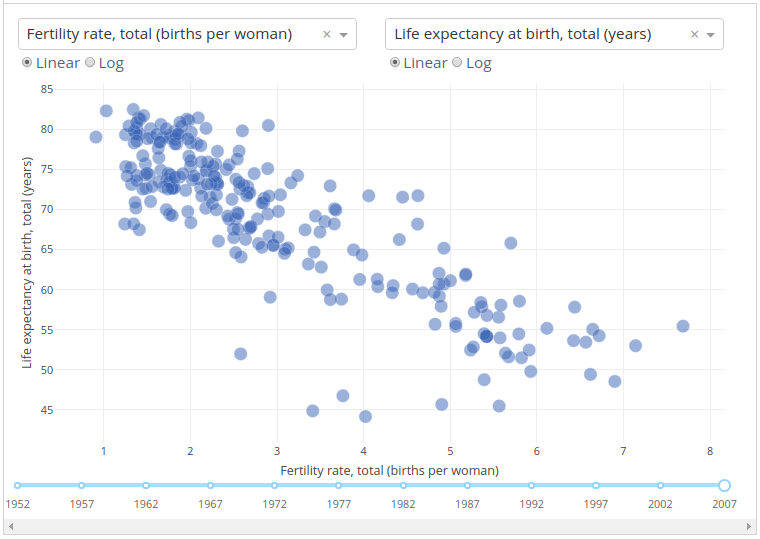
\includegraphics[scale=0.5]{dash}
	\caption{Contoh aplikasi web menggunakan Dash}
	\label{Dash}
\end{figure}

\subsubsection{ZeroMQ}
ZeroMQ adalah library untuk \textit{messaging} secara asinkron yang memiliki performa tinggi. ZeroMQ dapat digunakan untuk \textit{multi processing} dan \textit{multi threading}.
ZeroMQ memiliki API yang dirancang seperti soket Barkeley.
ZeroMQ menyediakan soket (semcam IP sederhana dan soket dengan domain UNIX), yang masing-masing dapat mewakili koneksi \textit{many-to-many} diantara endpoint. ZeroMQ melakukan pengiriman pesan menggunkan pola tertentu.
Pola dasar pengiriman pesan pada ZeroMQ:
\begin{enumerate}
	\item \textbf{Request-Reply}: menghubungkan antara klien dengan server. Komunikasi ini menggunakan prosedur \textit{request} dan \textit{response}.
	\item \textbf{Publish-Subscribe}: menghubungkan antara publisher dan subscriber. Komunikasi ini merupakan pola distribusi data.
	\item \textbf{Push-Pull}: menghubungkan node dalam pola fan-out/fan-in yang dapat memiliki beberapa step dan loop. Komunikasi ini merupakan pola distribusi dan pengumpulan data secara parallel. 
	\item \textbf{\textit{Exclusive pair}}: menghubungkan dua soket secara eksklusif.
\end{enumerate}
Pada ZeroMQ, protokol pengiriman pesan yang tersedia meliputi TCP, PGM (multicast), komunikasi \textit{inter-process} (IPC) dan komunikasi \textit{inter-thread} (ITC) \cite{ZeroMQ}.

\subsubsection{LabelImg}
LabelImg adalah alat untuk anotasi dan pelabelan \textit{bounding box} pada gambar. Alat ini ditulis dalam bahasa Python dan menggunakan Qt untuk antarmuka grafisnya. LabelImg mendukung 2 tipe anotasi yaitu PASCAL VOC dan YOLO. 
Anotasi untuk PASCAL disimpan dalam format XML, seperti format yang digunakan oleh ImageNet. Sedangkan anotasi YOLO akan disimpan dalam bentuk .txt \cite{LabelImg}

\end{document}
%\end{document}
